\section{Generovanie HDR obsahu}

Potom, ako je fotoaparátom zariadenia zachytená séria snímok s rôzným expozičným časom, je potrebné tieto
obrázky zlúčiť do jedného HDR obsahu. Celý algoritmus spájania série snímok je obsiahnutý v triede
\texttt{HDRController}, ktorý dekomponuje problém do troch tried spomenutých v tejto kapitole. Pri zápise rovníc
a v zdrojovom kóde aplikácie sa nachádzajú premenné, ktorých význam je stručne popísaný v kapitole
\ref{sec:Theory-Generating}.

\subsection{Výber vzorky pixelov pre získanie krivky odozvy}

Pred generovaním samotného HDR obsahu si musíme vyjadriť krivku odozvy fotoaparátu a to riešením kvadratickej
objektívnej funkcie \ref{eq:objFunction}. Teoreticky by sa na riešene tejto rovnice mohol vziať každý pixel, 
každej expozície, ale to by bolo na výpočet veľmi časovo a priestorovo náročné. My však nepotrebujeme všetky
dostupné pixely. Ak máme $P$ fotografií po $N$ pixelov, výsledná intenzita žiarenia $E_{i}$ bude mať $N$ hodnôt
a krivka odozvy $g$ $(Z_{max} - Z_{min})$ hodnôt. Na úspešné vyriešenie rovnice nám stačí
$N(P - 1) > (Z_{max} - Z_{min})$\cite{Debevec} hodnôt. Tieto hodnoty však musíme vhodne vybrať zo sekvencie
expozícii.

Medzi dostupné metódy výberu pixelov pre získanie krivky odozvy môžeme zaradiť:
\begin{description}
  \item [Vyhľadávanie vhodných oblastí] je metóda spomenutá v knihe od E. Reinharda \cite{HDRI}. Metóda vyberá
  vhodné oblasti pomocou vylučovania vzoriek - vhodná oblasť je jasnejšia ako akákoľvek oblasť z predchádzajúcich
  expozícií, neprekrýva žiadnu inú oblasť a~má malú odchýlku v jase vlastných pixelov. Takto sa vyberá dostatočný
  počet oblastí od najjasnejšej po najtmavšiu expozíciu. V prípade, že tmavšie expozície nevyužívajú celý rozsah
  jasu je ťažké nájsť oblasti, ktoré sú jasnejšie ako na predchádzajúcej expozícii. To nejako významne neovplyvní
  výsledok, ale je dôležité stanoviť limit pri vylučovaní oblastí na jednej expozícii, aby sa algoritmus nedostal
  do nekonečného cyklu.

  \item [Výber pixelov pomocou histogramu] spočíva vo vytvorení histogramu hodnôt a počtu pixelov s týmito
  hodnotami pre jednotlivé expozície. Z každého histogramu boli nás-ledne vybrané hodnoty, ktoré pixely najčastejšie
  nadobúdali. Problémom metódy však je, že pri najtmavších expozíciách sú vybrané samé čierne pixely a pri svetlých
  expozíciách je to naopak. Kód zobrazuje tvorbu histogramu vytvoreného z jasovej zložky obrazu.
\begin{lstlisting}[]
histogram = new int[256];

for (int i = 0; i < jasovaZlozka.length; i++) {
  histogram[jasovaZlozka[i]] += 1;
}
\end{lstlisting}
  
  \item [Pravidelne usporiadané pixely] získame vybraním každého $n$-tého pixelu v určitom smere. Vyberať je možné
  prechádzaním riadkov, stĺpcov alebo diagonál. Metóda je veľmi efektívna najmä pri vhodne zvolenom kroku
  
  \item [Náhodný výber pixelov] je najjednoduchšou a často aj dostatočne efektívnou metódou. Táto metóda je
  implementovaná v triede \texttt{SamplesSelector}, ktorá pri inicializovaní vyjadrí potrebný počet hodnôt pixelov
  potrebných pre vyriešenie kvadratickej objektívnej rovnice.
\begin{lstlisting}[]
List<Integer> vybraneIndexy = new ArrayList<>();
int i = 0;

while (vybraneIndexy.size() < velkostVzorky) {
  // nahodny index pixelu
  int index = (int) Math.floor(Math.random() * pocetPixelov);

  if (!vybraneIndexy.contains(index)) {
    // nahodne vybrany index nemame vo vybranych
    for (int j = 0; j < pocetFotografii; j++) {
      // ulozit pixel na vybranom indexe
      vzorkaPixelov[i][j] = images.get(j).getPixel(index);
    }
    vybraneIndexy.add(idx);
    i++;
  }
}
\end{lstlisting}
  Z dôvodu zamedzenia nežiadúcemu stavu, že bude
  viackrát náhodne vybraný práve jeden pixel (čo je pri počte pixelov na fotografii málo pravdepodobné),
  je definované pole vybraných indexov. Vhodný index je taký, ktorý sa nenachádza v poli už vybraných indexov.
\end{description}

\begin{figure}[t]
  \centering
  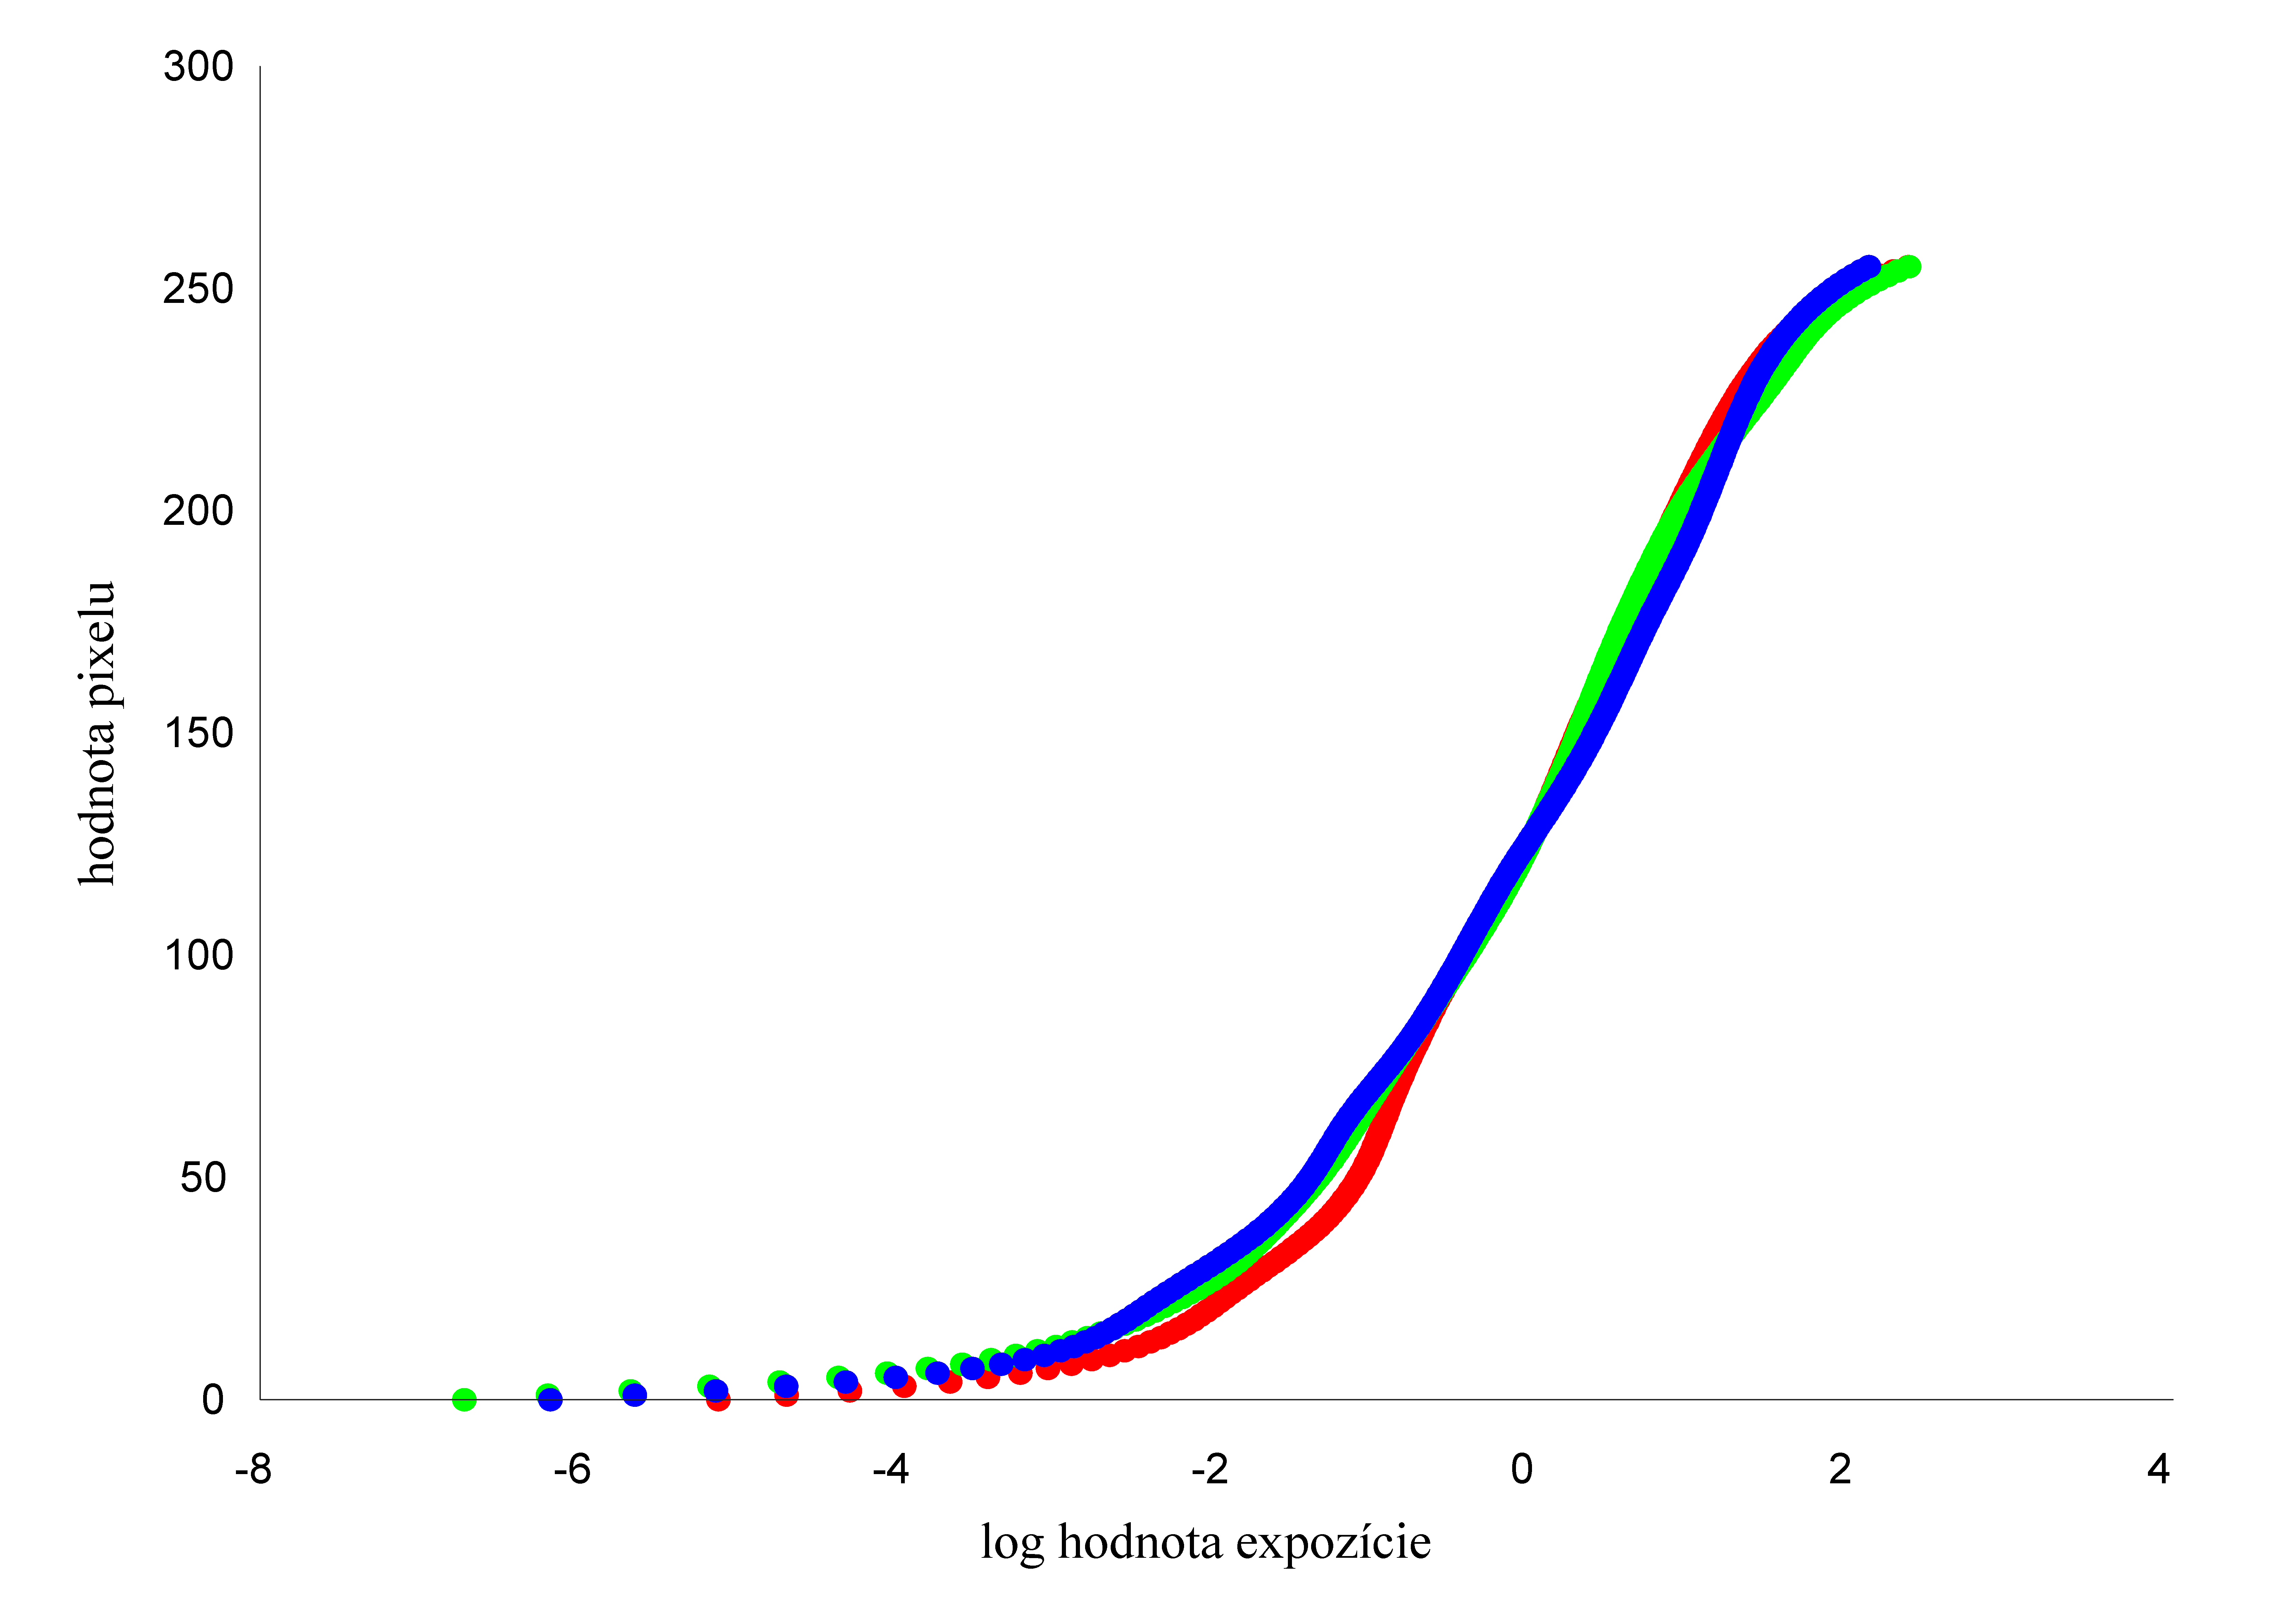
\includegraphics[width=0.9\textwidth]{figures/generating/octave-crf}
  \caption{Graf CRF kriviek jednotlivých farebných kanálov}
  \label{fig:octave_crf}
\end{figure}

\subsection{Získanie krivky odozvy fotoaparátu}

Ak máme vybrané dostatočné množstvo hodnôt, môžeme riešiť objektívnu kvadratickú rovnicu \ref{eq:objFunction}.
Rovnica je doplnená o váhovú funkciu \ref{eq:weightFunction}, pomocou ktorej dosiahneme, že hodnoty v okolí
$Z_{mid}$ budú mať väčšiu váhu ako hodnoty v okolí $Z_{min}$ a $Z_{max}$. $Z_{mid}$ je prostredná hodnota rozsahu
hodnôt pixelu, vyjadrená ako $Z_{mid} = \frac{1}{2}(Z_{min} + Z_{max})$. Túto hodnotu je potrebné nastaviť na 0.

\begin{equation} \label{eq:weightFunction}
  w(z)=
  \begin{cases}
    z - Z_{min}, & \text{pre}\ z \leq \frac{1}{2}(Z_{min} + Z_{max}) \\
    Z_{max} - z, & \text{pre}\ z > \frac{1}{2}(Z_{min} + Z_{max})
  \end{cases}
  \cite{Debevec}
\end{equation}

Keďže aplikácia pracuje s farebnými obrázkami, musíme vyjadriť krivku odozvy $g$ pre každý farebný kanál (obr. \ref{fig:octave_crf}).
Pridaním váhovej funkcie sa rovnica \ref{eq:objFunction} z podkapitoly \ref{sec:Theory-Generating} upraví na~tvar:
\begin{equation} \label{eq:rrFunction}
        \mathcal{O} = 
        \sum_{i=1}^{N}
        \sum_{j=1}^{P}
        \big (w(Z_{ij})[g(Z_{ij}) - \ln E_{i} - \ln \Delta t_{j}] \big )^{2}
        + \lambda
        \sum_{z=Z_{min} + 1}^{Z_{max} - 1}
        [w(z) g''(z)]^{2}
        \cite{Debevec}
\end{equation} 

Trieda \texttt{CRFRecover} implementuje riešenie tejto rovnice na základe ukážky \texttt{MATLAB} kódu od Paula
E. Debeveca a J. Malika\cite{Debevec}. Kód bol
debugovaný pomocou voľne šíriteľného softvéru GNU Octave\footnote{\url{www.gnu.org/software/octave/}}
a následne implementovaný v Jave. Na záver je potrebné vykonať dekompozíciu vytvorených matíc. Dekompozícia
je realizovaná pomocou metódy SVD\footnote{Singular-value decomposition},
z knižnice OpenCV.

\subsection{Vytvorenie funkcie žiarenia}

Ak už máme vyjadrenú krivku odozvy $g$, vieme ju použiť na prepočet hodnoty pixelu na~relatívnu hodnotu žiarenia.
Riešením rovnice \ref{eq:gFunction} a pridaním váhovej funkcie \ref{eq:weightFunction} získame rovnicu:
\begin{equation}
    \ln E_{i} = 
    \frac{
        \sum_{j=1}^{P}
        w(Z_{ij})(g(Z_{ij}) - \ln \Delta t_{j})
    }{
        \sum_{j=1}^{P}
        w(Z_{ij})
    }
    \cite{Debevec}
\end{equation}
Na generovanie HDR obsahu potrebujeme vyjadriť $\ln E_{i}$ pre každý pixel a každý farebný kanál. Vyjadrená
hodnota pixelu v logaritmickom tvare sa musí upraviť na základný tvar $E_{i}$ pomocou inverznej funkcie
$e^{x}$. Na záver sú tieho hodnoty funkcie žiarenia zlúčené do matice \texttt{org.opencv.core.Mat} typu
\texttt{CvType.CV\_32FC3}, čo značí maticu 32-bitových hodnôt s pohyblivou rádovou čiarkou pre 3 farebné kanály.
Tento algoritmus je implementovaný v~triede \texttt{HDRMerge}.
